\documentclass[12pt,a4paper]{article}
\usepackage{graphicx}
\usepackage{wrapfig}
\usepackage{textcomp}

\title{Praktikum Physik - Hydrodynamik}
\author{Simon Marti, Patricia Schwab, Mirco Kocher}
\date{23.03.2012}

\newcommand{\subscript}[1]{$_{#1}$}
\newcommand{\B}[1]{B\subscript{#1}}
\newcommand{\V}[1]{V\subscript{#1}}

\parindent=0pt 
\begin{document}
\maketitle


\section*{Ziel}
TODO

\section*{Motivation}
TODO

\section*{Theorie}
TODO

\section*{Experiment I}

\subsection*{Aufbau und Ablauf}
\begin{center}
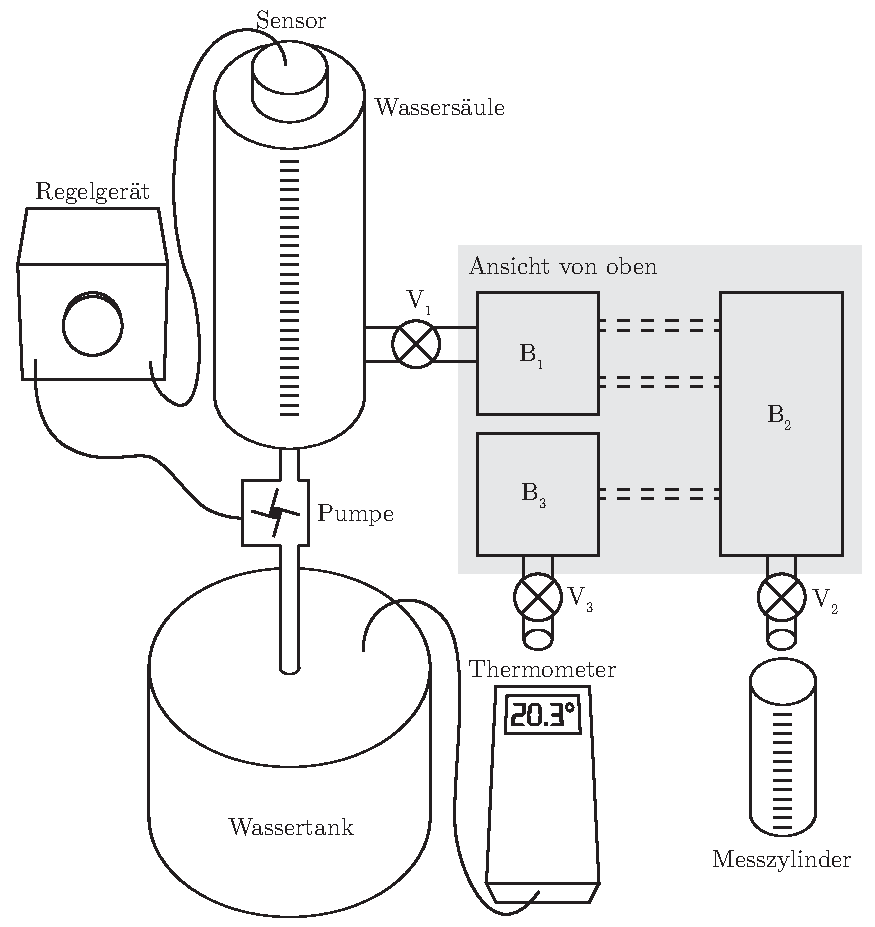
\includegraphics[width=11cm]{illustration.pdf}
\end{center}

Die aufgebaute Apparatur besteht aus wehreren Wasserbehältern die über R\"ohren und Schläuche miteinander verbunden sind. Zentral befinden sich drei Beh\"alter (\B{1}, \B{2} und \B{3}) die durch Kapillaren miteinander verbunden werden k\"onnen. An \B{2} und \B{3} befindet sich je ein Hahn durch welchen Wasser in einen Messzylinder geleitet werden kann (\V{2}, \V{3}). \B{1} ist mit einer Wassers\"aule verbunden die durch ein Regelgerät, welches mit einer Wasserpumpe und einem Wasserstand-Sensor verbunden ist, auf konstanter H\"ohe gehalten wird und oben offen ist. Das Wasser entnimmit die Pumpe aus einem offenen Beh\"alter in dem mithilfe eines elektronischen Thermometers die Wassertemperatur gemessen werden kann. Es befinden sich zusätzlich Entl\"uftungsventiele und Querverbindungen an den Beh\"altern die für die Versuche unwichtig sind und deshalb in der Grafik weggelassen wurden. Eine komplette \"Ubersicht der Ventiele findet sich im Script auf Abbildung 10.4.

Da die Vikosit\"at des Wassers von dessen Temperatur abh\"angt wird diese w\"ahrend der Durchf\"uhrung aller folgenden Augaben alle 15 Minuten gemessen.

\subsection*{Rohdaten}
\begin{tabular}{|l|l|}
\hline
$t$ [h]&$T$ [\textdegree C]\\
\hline
15:00&18.6\\
15:15&19.0\\
15:30&19.3\\
15:45&19.7\\
16:00&20.2\\
16:15&20.7\\
\hline
\end{tabular}


\section*{Experiment II}

\subsection*{Aufbau und Ablauf}

\subsection*{Rohdaten}
\subsection*{Rohdaten}
\begin{tabular}{|l|l|}
\hline
$h$ [cm]&$Q$ [ml/min]\\
\hline
50&33\\
59.7&38.5\\
55&36\\
46.4&31\\
38.7&26\\
31.6&21\\
20.6&14\\
\hline
\end{tabular}

\subsection*{Auswertung}


\section*{Experiment III}

\subsection*{Aufbau und Ablauf}

\subsection*{Rohdaten}
\begin{tabular}{|l|l|}
\hline
$d$ [mm]&$Q$ [ml/min]\\
\hline
1.01&33\\
0.61&5\\
0.84&17.25\\
1.23&65\\
\hline
\end{tabular}

\vspace{5pt}
$h$ = 50cm

\subsection*{Auswertung}


\section*{Experiment IV}

\subsection*{Aufbau und Ablauf}

\subsection*{Rohdaten}

$d_1$ = 1.01mm

$d_2$ = 1.00mm

$Q_{Parallel}$ = 68ml/min

$Q_{Seriell}$ = 17.25ml/min

$Q_{1}$ = 33ml/min

$Q_{2}$ = 33ml/min

\subsection*{Auswertung}


\section*{Experiment V}

\subsection*{Aufbau und Ablauf}

\subsection*{Rohdaten}
\begin{tabular}{|l|l|}
\hline
$h$ [cm]&$Q$ [ml/min]\\
\hline
59.7&274\\
42.8&242.5\\
28&190\\
11.8&97.5\\
35.2&220\\
50.5&256\\
20.4&150\\
15.4&120\\
25.5&178\\
30.8&202.5\\
\hline
\end{tabular}

\subsection*{Auswertung}


\section*{Diskussion}


\end{document}